\chapter{Softwarekomponenten}

\section{Entwicklungsumgebungen}

Zu Beginn des Projekts wurden zwei gängige Entwicklungsumgebungen für die Programmierung von Mikrocontrollern evaluiert: die klassische \textit{Arduino IDE}, welche auch von den betreuenden Dozierenden empfohlen wurde, sowie die moderne, zunehmend verbreitete \textit{PlatformIO}-Erweiterung für Visual Studio Code.
Im Projektteam wird plattformübergreifend mit Linux, Windows 10 und Windows 11 gearbeitet. Beide Entwicklungsumgebungen sind grundsätzlich mit allen eingesetzten Betriebssystemen kompatibel. Zur Prüfung der technischen Umsetzbarkeit wurden zwei separate Repositories eingerichtet, in denen jeweils einfache Testprojekte zur Ansteuerung eines ESP32 implementiert wurden.
Beide IDEs konnten den Mikrocontroller erfolgreich ansprechen. PlatformIO bietet durch seine deklarative Verwaltung von Bibliotheken und Abhängigkeiten Vorteile in Bezug auf Reproduzierbarkeit und Build-Konsistenz. In der Praxis kam es jedoch auf einem System im Team zu anhaltenden technischen Problemen mit PlatformIO, die nicht zufriedenstellend gelöst werden konnten.
Um eine einheitliche und zuverlässige Entwicklungsgrundlage für alle Teammitglieder sicherzustellen, fiel die Entscheidung letztlich zugunsten der \textit{Arduino IDE}. Diese ermöglicht eine barrierefreie Mitarbeit aller Beteiligten, auch wenn sie im Funktionsumfang nicht ganz an PlatformIO heranreicht.

\section{Kommunikationsmethode}
ESP-NOW wurde ausgewählt, da es im Vergleich zu anderen Protokollen einen deutlich geringeren Overhead besitzt und dadurch eine schnellere und effizientere Datenübertragung ermöglicht. Die Struktur ist weniger komplex, was die Implementierung vereinfacht und die Fehleranfälligkeit reduziert. 
Dadurch wird das System insgesamt robuster und zuverlässiger:
ESP-Now ist ein Kommunikationsprotokoll von Espressif, das speziell für die ESP32- und ESP8266-Chips entwickelt wurde. Es verwendet die 2,4 Ghz Frequenz, welche eigentlich für WiFi Kommunikation verwendet wird. 
Im Gegensatz zu anderen Protokollen sind die Nachrichten auf Schicht 2 des ISO-OSI-Modells. Keine IP-Adressen sondern nur MAC-Adressen. Die ESPs müssen sich dafür im gleichen Kanal befinden. Die 2,4 Ghz Frequenz hat grundsätzlich nur 3 Nutzbare Kanäle. 
Der zu verwendene Kanal muss von dem "AI401" Wlan Netz übernommen werden.Es ist mit relativ wenig Code möglich eine große Menge an Daten in sehr Kurzen Zeitabschnitten zu senden. Theoretisch ist eine Datenübertragung von 1 bis 2 Mbps möglich. 
Die Nachrichtenlänge ist auf 250 Byte pro Paket beschränkt. Da unsere Nachrichten nur wenige Bit lang sind, haben wir hier keine Probleme. 
Das Protokoll hat keine festgelegten Sender/Empfänger Rollen. Jeder ESP kann senden und empfangen. In unserem Beispiel senden aber 3 ESPs und ein Edge-Device empfängt alle Daten. 
Es wird 10 mal pro Sekunde der Lautstärkepegel erfasst und gesendet.


\section{Frontend}
\subsection{Technologieauswahl}
Für die Umsetzung des Frontends wurde das Framework \textit{Angular} gewählt. 
Diese netschiedung basiert auf technischen Faktoren und persönlichen Preferenzen. 
Angular bietet eine klare Struktur durch komponentenbasiertes Design und ist für die moderne Webentwicklung gut geeignet.
Es erleichtert die Wiederverwendbarkeit von eigenen aber auch externen UI-Elementen und unterstützt eine saubere Trennung von Logik und Darstellung. 

Im Vergleich dazu ist \textit{React} ein von Meta entwickeltes UI-Framework. 
\textit{Angular} und \textit{React} haben beide eine komponentenbasierte Architektur. 
Diese Komponenten sind innerhalb anderer Komponenten wiederverwendbar und somit endlos wiederverwertbar. 
Beide sind Open Source. Daher haben React und Angular große Entwicklergemeinschaften, die die Ressourcen regelmäßig erweitern.
Angular ist ein vollwertiges Framework, während React eine JavaScript-Bibliothek ist. 
Deshalb muss React mit einem Framework gepaart werden, um eine schnelle, schöne und kompatible Benutzeroberfläche zu erstellen. 
\cite{kinsta2023angularvreact}

Da außerdem im Team bereits umfangreiche Erfahrung mit diesem Framework vorhanden war, fiel die Entscheidung zugunsten von Angular.
Das Frontend läuft in einem eigenen Docker-Container und kommuniziert, über ein internes Netzwerk, mit dem separat laufenden Backend-Container. 
So bleibt die Architektur modular, skalierbar und einfach wartbar.

\subsection{Umsetzungsplan}
Während der Entwicklung wurde ein einfaches Frontend zu Testzwecken angelegt. 
Deshalb soll nun ein Plan entwickelt werden, wie die Benutzeroberfläche aussehen soll und welche Funktionen sie bieten soll:
\begin{center}
  \includegraphics[width=1\textwidth]{../images/UI/SkizzeUI.png}
\end{center}
In dieser Skizze wurden die Grundfunktionen der Benutzeroberfläche festgelegt und die Anordnung der einzelnen Elemente skizziert.
Über eine Navbar an der linken Seite kann zwischen den einzelnen Seiten gewechselt werden. 
Auf der Hauptseite wird eine Heatmap angezeigt, die die Lautstärkeverteiung im Vorlesungsraum räumlich darstellt, wobei mit einem Dropdown-Menü der anzuzueigende Zeitraum ausgewählt werden kann.
Durch den ausgewählten Zeitraum kann anschließend mit einem Schieberegler die Zeit ausgewählt werden, für die die Lautstärke angezeigt werden soll.
Im nächsten Nav-Item sollen die einzelnen 2D-Grafen der jeweiligen Sensoren angezeigt werden. 
Das dritte Nav-Item soll einen tabellarischen Überblick über die gesammelten Daten geben, die in der Datenbank gespeichert sind.
Die Nvabar bietet Raum für zukünfitge Erweiterungen.

\subsection{Umsetzung}
Auf Grundlage dieser Skizze wurde das Frontend und UI efolgreich umgesetzt.
So hat man nun eine übersichtliche Homepage, die auf alle Elemente verweist, welche auch in der interaktiven Navbar zu finden sind.
Als kleines AddOn wurde unteranderem hierfür ein "AudiTim" Logo entworfen, was den ikonischen Hirsch mit dem vernetzten Geweih und den Audiowellen verknüpft, sowie eine Light- und Darkmode Funktionalität implementiert.
\begin{center}
  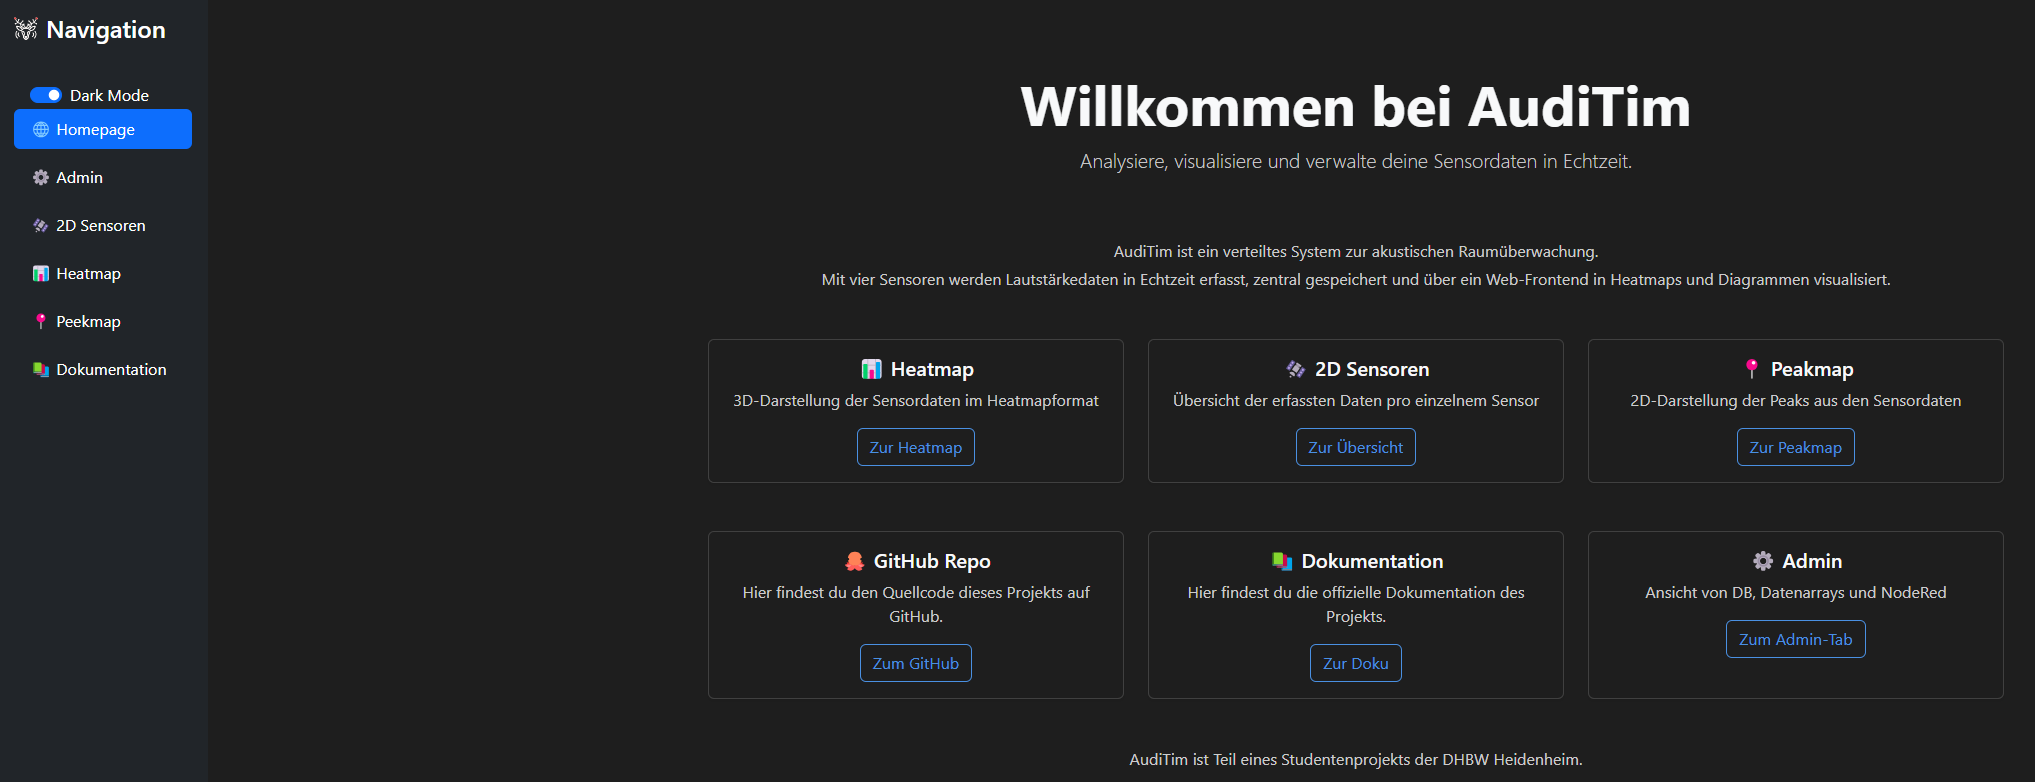
\includegraphics[width=1\textwidth]{../images/UI/homepage.png}
\end{center}

Auch im Screenshot zu sehen, sind die schlussendlich umgesetzten Seiten; Heatmap, 2D-Sensoren, Peakmap, Github Repo, Dokumentation und Admin. 
Für diese Seiten wurden die in der Skizze angedachten Funktionen erfolgreich umgesetzt und flexibel während der Entwicklung angepasst und erweitert.

So zeigt die Admin-Seite nun eine Übersicht über die verbundenen Container und Elemte sowie deren Status an:
\begin{center}
  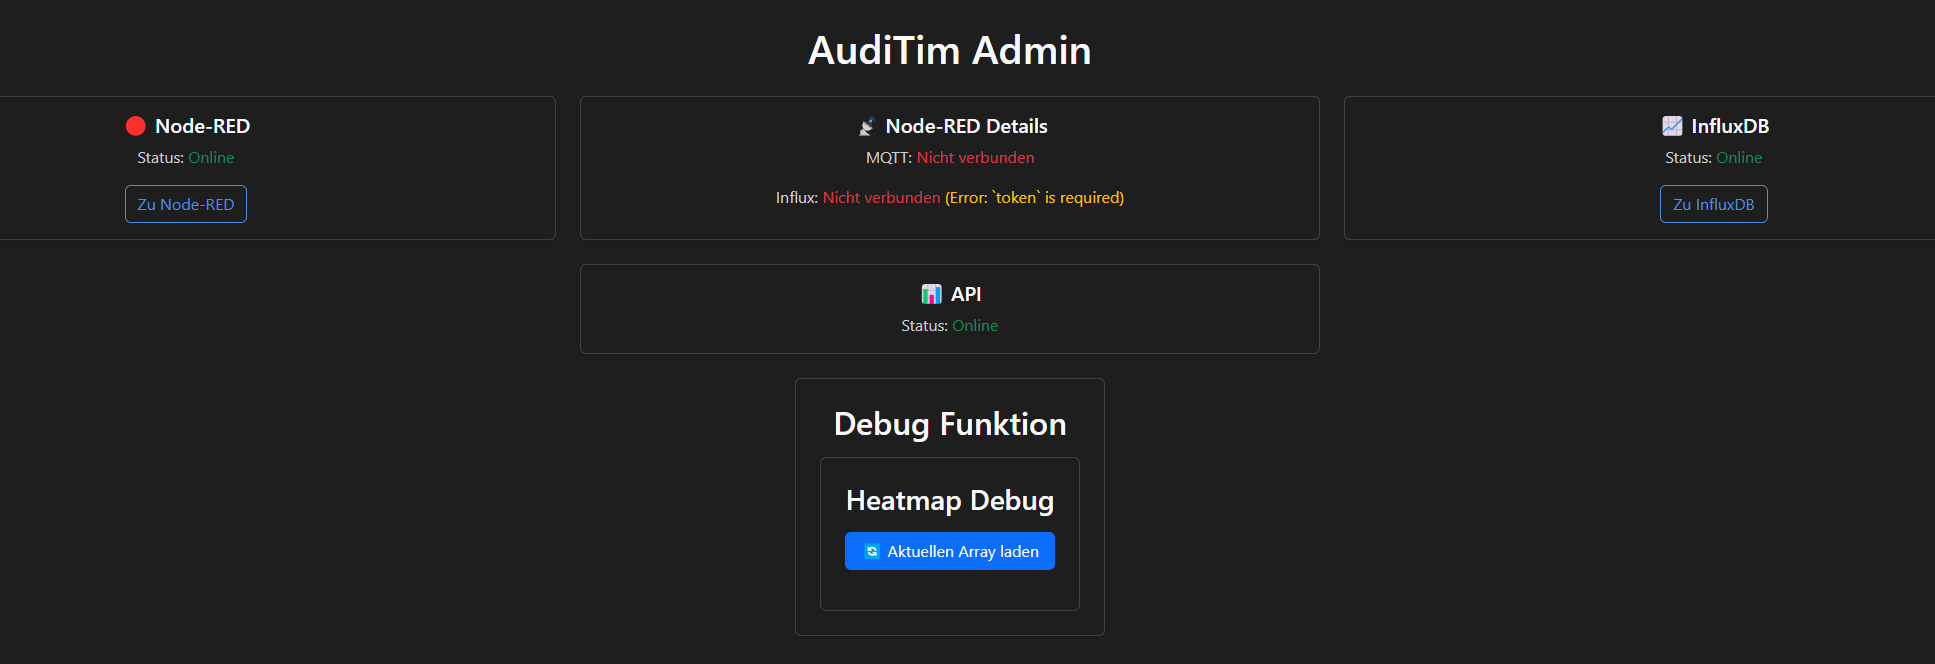
\includegraphics[width=1\textwidth]{../images/UI/admin.png}
\end{center}

Die 2D-Sensoren-Seite zeigt die einzelnen Sensorwerte in übersichtlichen Liniendiagrammen an, wobei man zwischen einem ausgewählten Zeitraum und einem Live-Modus wechseln kann:
\begin{center}
  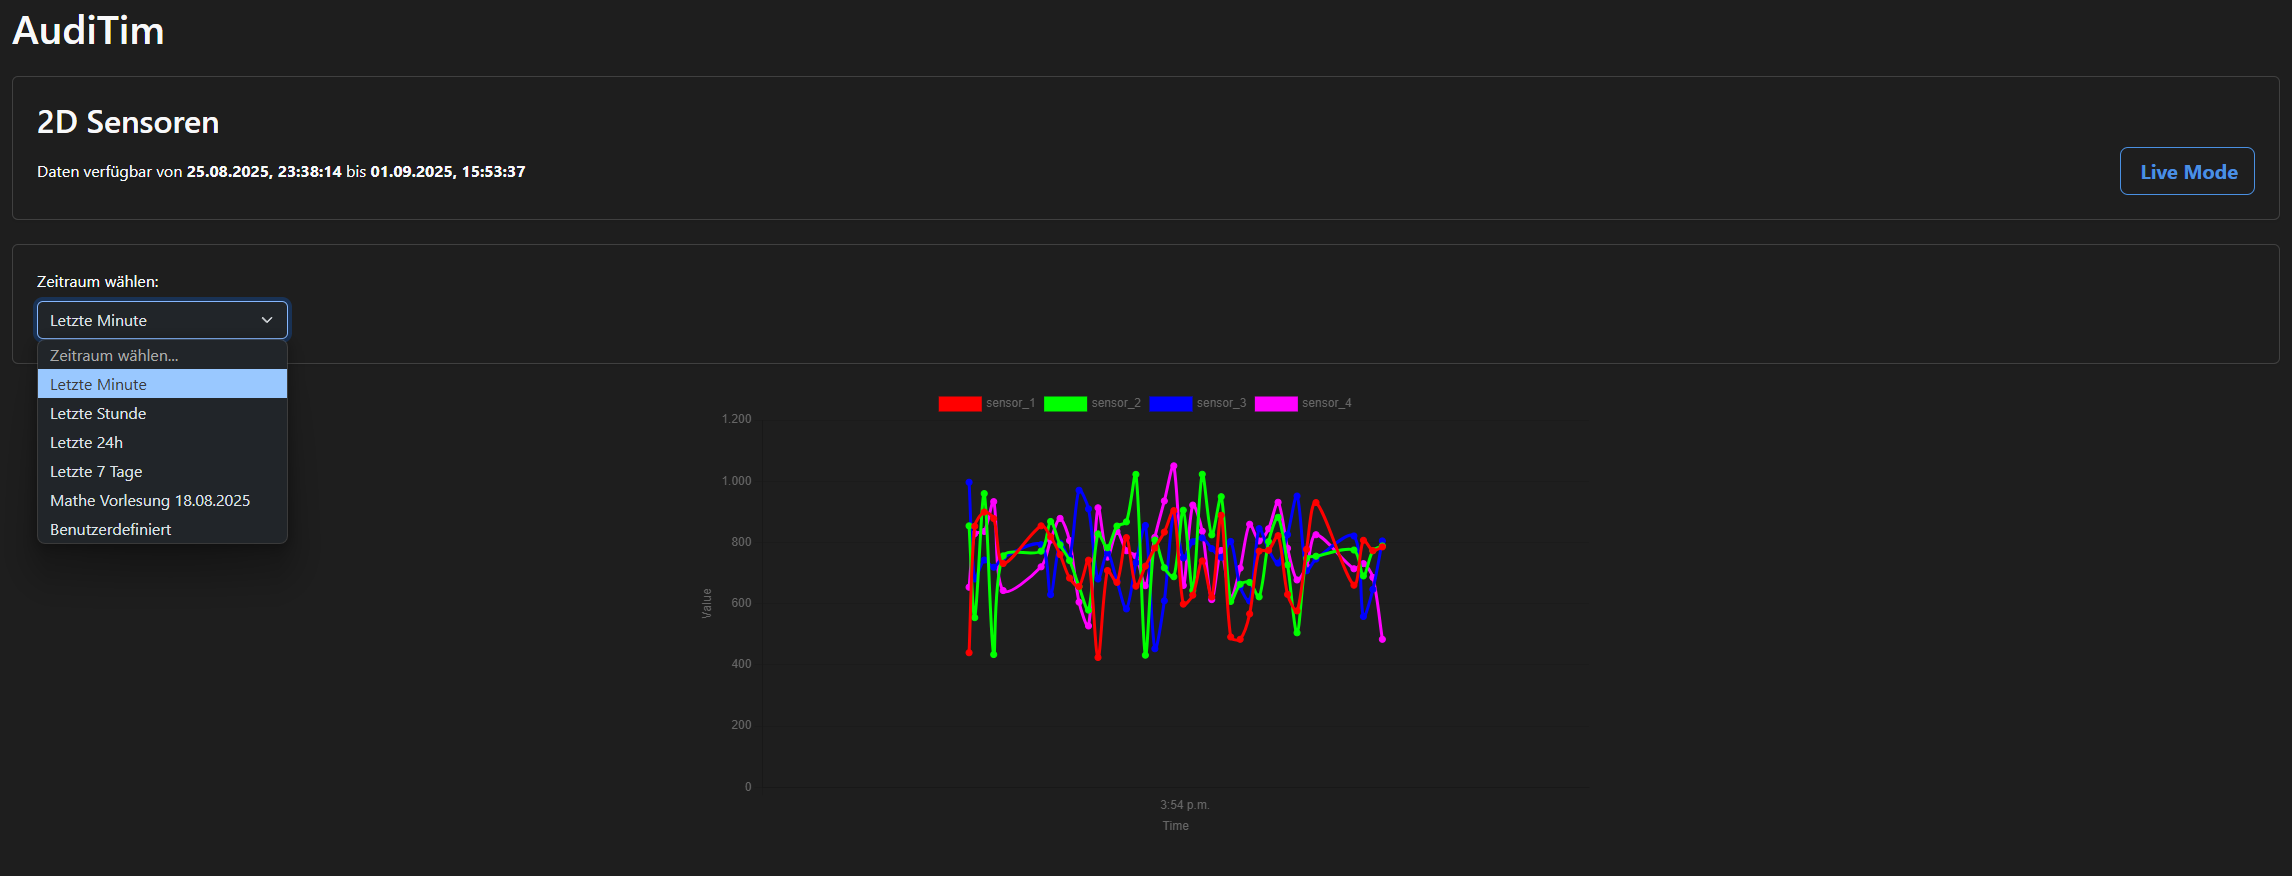
\includegraphics[width=1\textwidth]{../images/UI/zweid.png}
\end{center}

Auch die Heatmap-Seite zeigt die Auswahl zwischen einem ausgewählten Zeitraum und einem Live-Modus, sowie einen Average-Modus, in dem die durchschnittliche Lautstärke über den ausgewählten Zeitraum angezeigt wird. 
Mit einem Schieberegler kann die Zeit innerhalb des ausgewählten Zeitraums angepasst werden und gegenenenfalls eine Animation gestartet werden, die die Lautstärkeverteilung über den Zeitraum hinweg anzeigt.
Außerdem wurde das in "4.5 3D-Raummodellierung" beschriebene 3D-Modell des Raumes als Hintergrundbild für die Heatmap verwendet, um eine realistische Darstellung zu ermöglichen:
\begin{center}
  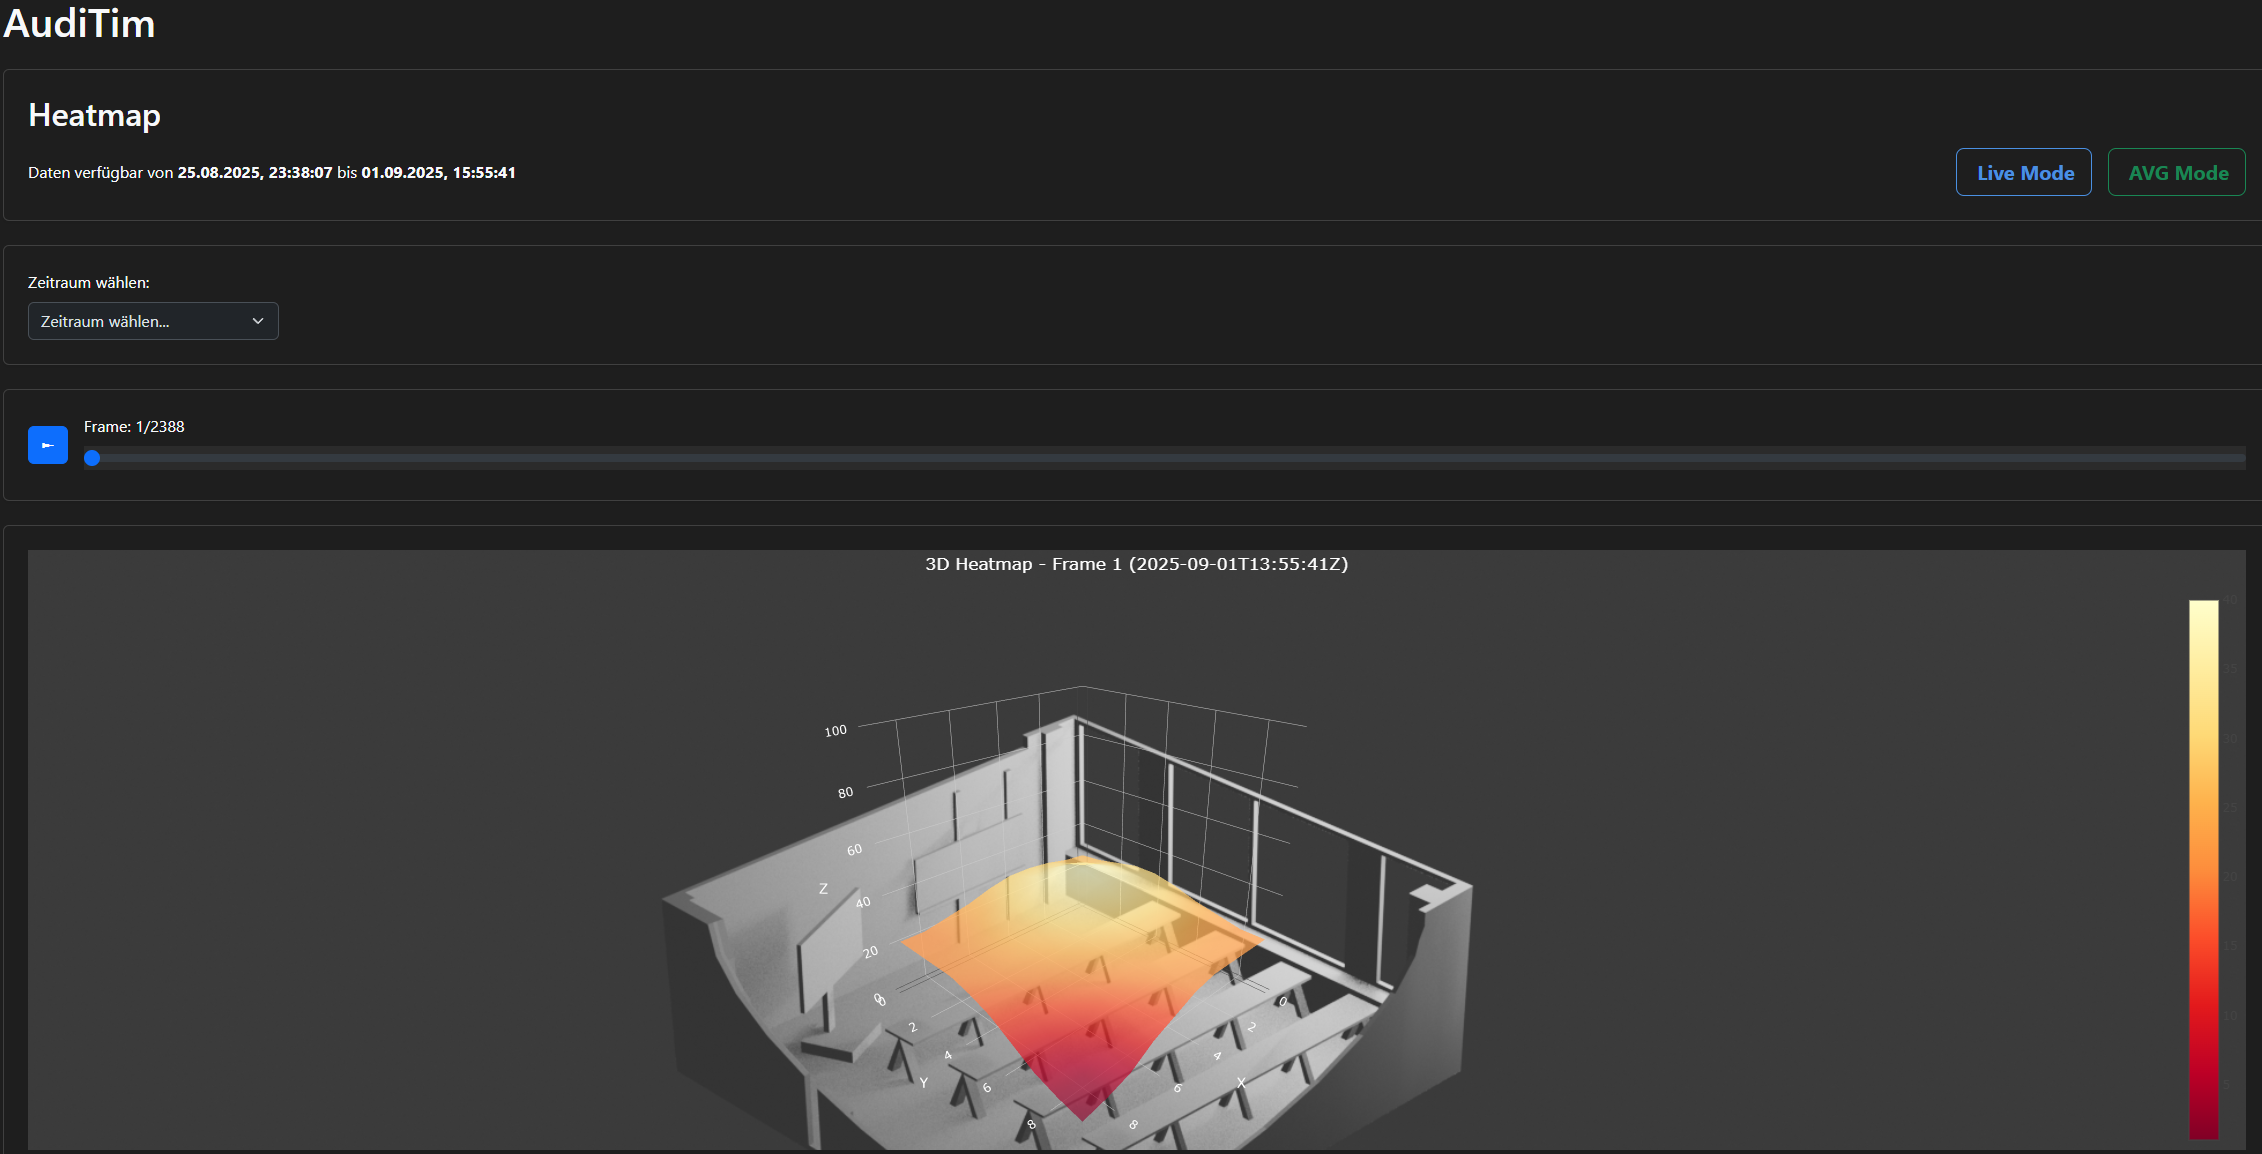
\includegraphics[width=1\textwidth]{../images/UI/heatmap.png}
\end{center}

Dieses 3D-Modell wurde auch für die Peakmap-Seite verwendet, auf der die Spitzenwerte der Sensoren über den ausgewählten Zeitraum angezeigt werden:
\begin{center}
  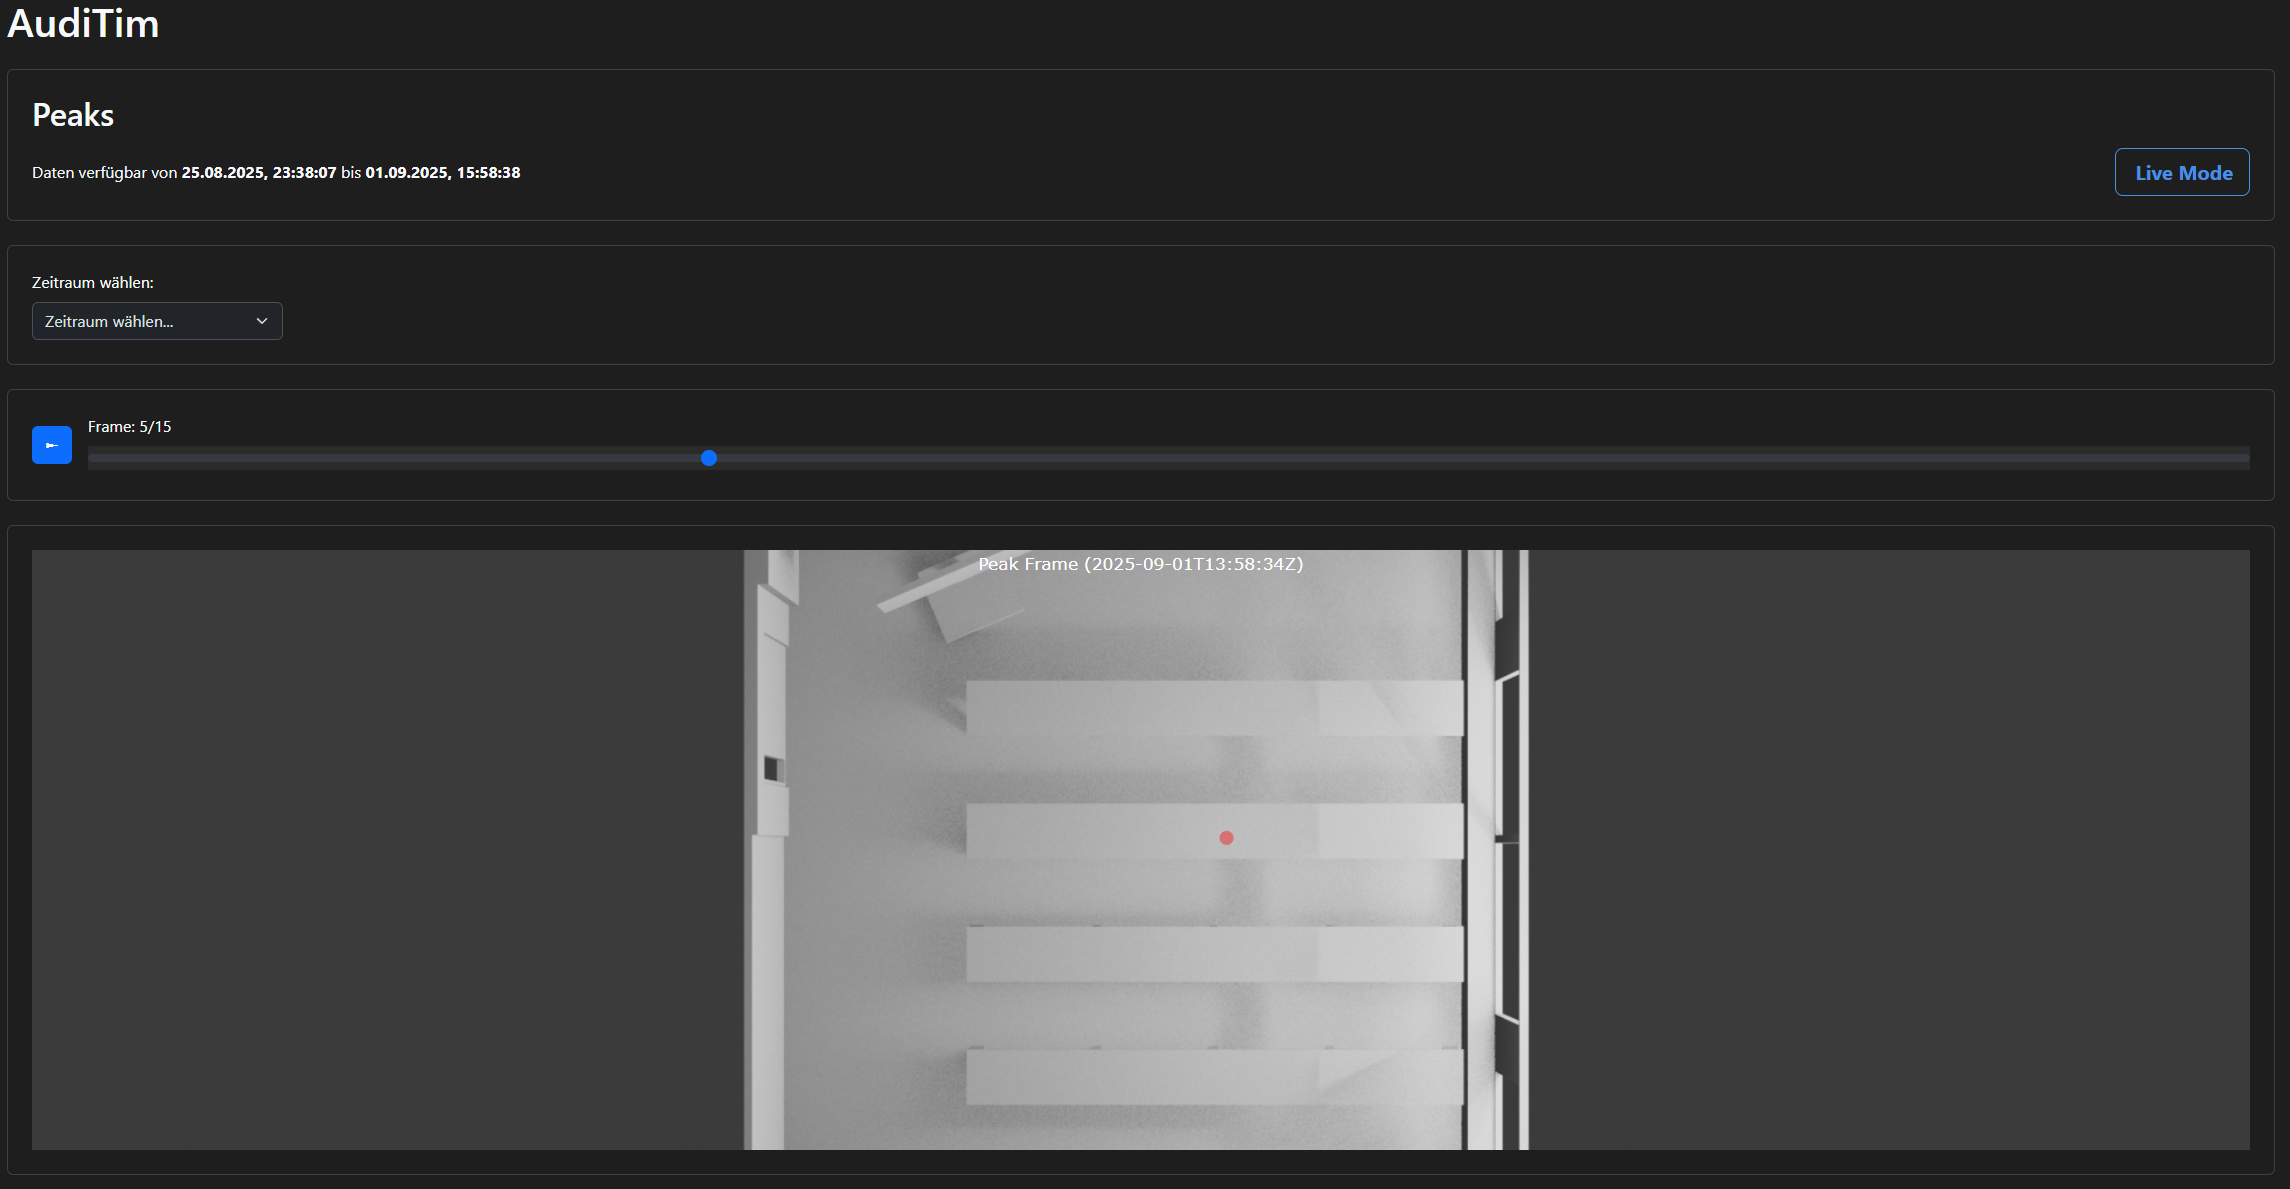
\includegraphics[width=1\textwidth]{../images/UI/peak.png}
\end{center}

Und zu guter Letzt zeigt die Dokumentation-Seite diese Dokumentation, die sie hier gerade lesen, in einem eingebetteten PDF-Viewer an. 

\subsection{Testing}
Für die Umsetzung des automatisierten Testings wurde Playwright eingesetzt. Die Auswahl dieses Frameworks erfolgte nach einer vergleichenden Analyse. Dabei wurde Playwright von einem Teammitglied im Rahmen einer Projektarbeit mit einem ähnlichen Anwendungsfall ausführlich evaluiert und als am geeignetsten bewertet. Ausschlaggebend hierfür waren insbesondere die breite Browserunterstützung, die integrierten Funktionen für End-to-End-Tests sowie die hohe Stabilität und Geschwindigkeit der Testausführung.

Durch den Einsatz von Playwright konnte die Konsistenz der Benutzeroberfläche (UI) zuverlässig sichergestellt werden. Die automatisierten Tests ermöglichen es, Interaktionen und Darstellungsvarianten reproduzierbar zu prüfen und so frühzeitig Abweichungen oder Fehler zu erkennen. Auf diese Weise trägt das Testing wesentlich zur Qualitätssicherung und Nachhaltigkeit der entwickelten Lösung bei.



\section{Backend}
Das Backend wurde mit Node.js und dem minimalistischen Framework Express.js umgesetzt. 
Express ist das am weitesten verbreitete Node.js-Framework für Webserver und APIs. 
Es bietet eine ausgereifte Middleware-Architektur, die sehr flexibel und modular ist. 
Im Vergleich zu ähnlich minimalistischen Frameworks wie Koa, 
das von den gleichen Entwicklern stammt, 
bietet Express mehr out-of-the-box Funktionalitäten und eine größere Community mit umfangreichen Plugins und Support. \cite{betterstack2025koavsexpress,appventurez2025nodejsframework}

Koa hingegen ist moderner und basiert stärker auf ES6 Features wie async/await, was den Code oft sauberer macht. 
Allerdings ist Koa weniger „batteries included“ und erfordert mehr Initialaufwand und zusätzliche Libraries, 
um Funktionen bereitzustellen, die Express standardmäßig mitbringt. 
Für dieses Projekt, welches einen schnellen Einstieg, umfangreiche Dokumentation und stabile Middleware braucht, 
ist Express daher die pragmatischere Wahl.
Zudem sind Gruppenmitglieder bereits mit Express vertraut, was die Einarbeitungszeit verkürzt und die Produktivität steigert. 

Die Anbindung an eine InfluxDB erfolgt über die offizielle Client-Bibliothek. 
Neben dem Abrufen historischer Sensorwerte werden auch Funktionen zum Schreiben von Dummy-Daten bereitgestellt.
Diese werden, solange die Verbindung zu den wirklichen Sensorwerten noch nicht hergestellt ist, zum Testen verwendet.

Für die Speicherung der Sensordaten wurde InfluxDB gewählt. 
Eine Zeitreihen-Datenbank, die speziell für viele konsekutive Datenströme optimiert ist. 
InfluxDB bietet eine simple API und gutes visuelles UI, ohne dass viel Konfiguration nötig ist.
Im Vergleich zu einer relationalen Datenbank wie TimescaleDB, die auf PostgreSQL basiert,
ist InfluxDB deutlich einfacher zu handhaben und benötigt weniger Overhead für die Konfiguration.
Um eine TimescaleDB sicher zum laufen zu bringen, sind komplexe Zugriff-Skripte benötigt, um die Benutzer zu verwalten.
InfluxDB hingegen arbeitet mit einem einfachen Benutzer- und Rollenkonzept. 
Auch für die API-Authentifizierung ist InfluxDB mithilfe von Tokens und Secrets deutlich einfacher zu konfigurieren.
Der Rationale Aspekt einer traditionellen ist sicherlich in vieler Hinsicht nützlich, wird aber in diesem Projekt nicht benötigt.
Eine nahtlosen Integration in das Node.js-Backend ist mit der offiziellen InfluxDB-Bibliothek kein Problem.
InfluxDB wurde uns initial von den "Verteilten Systeme"-Dozenten ausdrücklich empfohlen, da wir viele Zeitwerte speichern und analysieren wollen.

\subsubsection*{Berechnung des Speicherplatzbedarfs für InfluxDB}

Zur Abschätzung des benötigten Speicherplatzes in InfluxDB betrachten wir die anfallenden Sensordaten pro Stunde.  

\paragraph{Rohdaten}  
Pro Sekunde werden \textbf{10 Messungen} von \textbf{4 Sensoren} erfasst, wobei jeder Wert als \texttt{double} (64\,Bit = 8\,Byte) gespeichert wird.  
Damit ergibt sich:  

\[
10 \times 4 \times 8 \,\text{Byte} \times 60 \times 60 
= 1{,}152{,}000 \,\text{Byte} \approx 1.1 \,\text{MB/h}
\]

\paragraph{Base64-kodierte Daten}  
Wird der Algorithmus auf die Sensordaten angewendet, erzeugt er daraus ein 10x10-Array mit Werten im Bereich von 0 bis 255. Dieses Array wird anschließend kodiert. Durch die Base64-Kodierung entsteht dabei ein Overhead von etwa 36\%. Für die Datenmenge ergibt sich pro Sekunde:  

\[
800 \,\text{Bit} = 100 \,\text{Byte} \quad \Rightarrow \quad 
\text{mit Overhead} \approx 136 \,\text{Byte}
\]

Somit pro Stunde:  

\[
136 \,\text{Byte} \times 60 \times 60 
= 489{,}600 \,\text{Byte} \approx 470 \,\text{KB/h}
\]

\paragraph{Fazit}  
Für die Speicherung in InfluxDB müssen daher pro Stunde etwa  
\[
1.1\,\text{MB (Rohdaten)} + 0.47\,\text{MB (Base64)} \approx 1.6\,\text{MB/h}
\]  
eingeplant werden.


Das Backend ist ebenfalls in einem eigenen Docker-Container gekapselt. 
Die Kommunikation mit dem Frontend erfolgt über definierte HTTP-Endpunkte im Container-Netzwerk. 
Diese Trennung verbessert die Wartbarkeit und erlaubt eine flexible Skalierung beider Komponenten unabhängig voneinander.

\section{MQTT Subscriber}
Um den Datenfluss zu verfollständigen fehlt eine Brücke zwischen dem MQTT Server und der InfluxDB. 
Hierfür wird ein sogenannter MQTT-Subscriber benötigt, der die Daten vom MQTT-Broker abonniert und in die InfluxDB schreibt.
Technisch gesehen kann dies mit einer vielzahl von Frameworks / Sprachen / Tools umgesetzt werden. 
Zum Beispiel mit Python, Node.js, Golang oder auch Java.
Wir haben uns für Node-RED entschieden, da es eine einfache und schnelle Möglichkeit bietet, um Daten von MQTT zu InfluxDB zu übertragen.
Node-RED ist eine visuelle Programmierumgebung, die auf Node.js basiert und es ermöglicht, Datenströme einfach zu verarbeiten und zu transformieren.
Besonders das debugging und die Visualisierung der Datenströme ist in Node-RED sehr einfach und intuitiv.
\cite{nodered2023docs}

Im Vergleich zu z.B. einem Python-Skript ist Node-RED deutlich einfacher zu handhaben.
Natürlich ist Node-RED nicht so performant oder bietet dieselbe Flexibilität und Kontrolle wie ein selbstgeschriebenes Skript,
ist aber dafür deutlich einfacher zu konfigurieren und zu warten.
Besonders in unserem spezifischen Fall, wo wenig Kontrolle über den schlussendlichen Server besteht, ist Node-RED eine gute Wahl.
Eine automatische Ausführung von Skripten ist beinahe unmöglich, das keine Kontrolle über Sudo-Level Systemdiensten besteht.

\subsection{NodeRED Umsetzung}
Node-RED stellte sich als eine gute Entscheidung heraus, um den Flow zwischen MQTT und InfluxDB zu realisieren, und aber auch um bspw. Statusanfragen für die Admin-Seite zu beantworten.
Das einzige Manko war das ständige Erneuern der Tokens für die InfluxDB, da Node-RED keine Möglichkeit bietet, Umgebungsvariablen zu verwenden.
Schlussendlich entstand ein gut-funktionierender Flow:
\begin{center}
  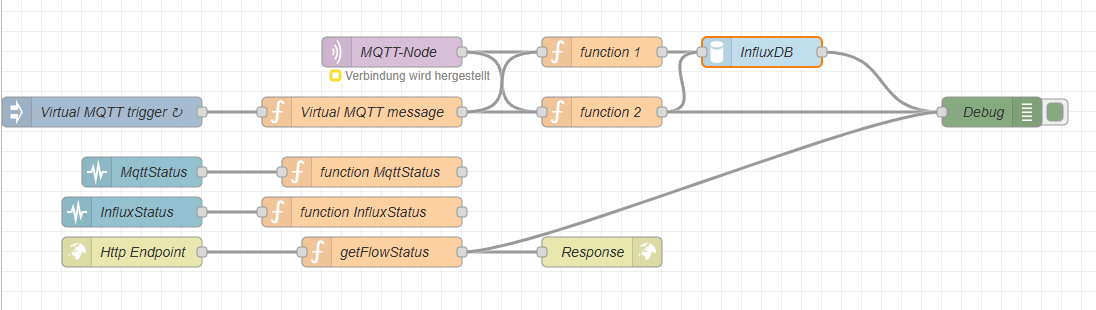
\includegraphics[width=1\textwidth]{../images/UI/flow.png}
\end{center}


